\chapter{\emph{AI Muse}, herramienta en {Python} para la interacción en vivo con \gls{llm} en entornos de \emph{live coding}}
\label{chap:ai_muse}

% \defaultFontEpigraph{One Model Is All You Need}{\cite{grahamOneModelAll2022}}
\defaultFontEpigraph{One Model Is All You Need}{Graham y cols. (2022)}

En este capítulo pasamos a describir la herramienta \emph{AI Muse}, creada durante este trabajo, a la cual nos referimos en el capítulo anterior (véase sección \ref{sec:generacion_automatica_codigo_tidal_cycles}), detallando su funcionamiento, diversas cuestiones de su implementación y los resultados de su utilización.

\section{Descripción general de la herramienta}

\emph{AI Muse} es una herramienta de interacción con modelos de lenguaje en entornos de \emph{live coding}. Está escrita en Python y se comunica con la API de OpenAI. Permite ejecutar código de SuperCollider y de Tidal Cycles. Además, tiene un archivo de configuración en formato JSON, así como un conjunto de comandos para modificar en vivo los parámetros de la configuración. Aunque está pensada para la utilización de modelos de OpenAI, esta librería permite eventualmente comunicarse con otros modelos de lenguaje incluso en local, detalle que no ha sido explorado en este trabajo.

\section{¿Por qué un entorno de \emph{live coding}?}

El \emph{live coding} es el arte de programar música en tiempo real, constituyéndose así como un espacio de experimentación y creación artística que fusiona el campo de la programación con el de la interpretación musical y la improvisación. Por su naturaleza, esta práctica brinda una plataforma ideal para explorar las posibilidades que la interacción con modelos de lenguaje de forma automatizada puede ofrecer.

Dado su carácter improvisatorio, no se limita a estructuras musicales preestablecidas. Esta flexibilidad en la forma implica menores restricciones temporales en comparación con la composición musical tradicional, lo cual se alinea perfectamente con los hallazgos de fases previas de nuestro trabajo. En dichas etapas, se evidenció que los modelos de lenguaje contemporáneos son más eficientes con fragmentos de código de tamaño reducido. Este enfoque creativo, sumado a las ventajas de Tidal Cycles en términos de fiabilidad del código y tolerancia a fallos, ha propiciado el desarrollo de \emph{AI Muse} como una herramienta de experimentación.


\section{Integración de la API de OpenAI}

\emph{AI Muse} integra dos posibles interacciones que OpenAI permite con su API: utilización modelos de chatbot y de sistemas de \gls{rag}\footnote{Los llamados \emph{Assistants} por OpenAI.}. La primera modalidad es la más sencilla, ya que se trata de realizar conversaciones con el modelo. En este caso, cada petición se limita a un prompt general de sistema unido al archivo actual con todo el código generado, de forma que el modelo pueda genera el siguiente bloque de código.

La diferencia crucial con scripts previos en este trabajo (véase sección \ref{sec:generacion_automatica_codigo_tidal_cycles}) es que es el propio usuario quien decide cuándo hacer una petición a la API, en lugar de estar automatizado. La acción elegida para hacer esta petición es la de guardar el archivo. De esta forma, el programa puede ser utilizado en cualquier editor de textos, y no está limitado a un entorno de desarrollo concreto ni al uso de \emph{plugins} o extensiones. En este caso, todo el programa ha sido escrito y testado en Visual Studio Code, pero eventualmente podría ser utilizado en cualquier otro editor de textos.


\section{Lenguajes de programación musical disponibles}

En un primer momento se implementó únicamente la posibilidad de ejecutar código de Tidal Cycles. Posteriormente, se añadió el soporte para SuperCollider, aprovechando las clases que este lenguaje ofrece para el \emph{live coding}. En ambos casos se ofrece la posibilidad de que sea el propio programa el que se ocupe de llamar a los binarios de los propios lenguajes, o que este código sea ejecutado por el usuario por otros medios (uso de plugins o de entornos de desarrollo específicos).


\section{Flujo de trabajo}

El flujo de trabajo típico de \emph{AI Muse} es el siguiente (cfr. Figura \ref{fig:ai_muse_flow}):

\begin{enumerate}
    \item El usuario ejecuta el programa. Automáticamente se creará un archivo en texto plano con la extensión adecuada (actualmente, \texttt{.tidal} o \texttt{.sc}, para Tidal Cycles y SuperCollider, respectivamente) para interactuar.
    \item El usuario abre un archivo de código en un editor de texto.
    \item \label{item:paso_write_code} El usuario puede escribir código musical, un comando de sistema o un simple comentario-mensaje para el modelo.
    \item Al guardar el archivo, \emph{AI Muse} lee el archivo y lo envía a la API de OpenAI. Adicionalmente, ejecuta los comandos nuevos escritos en el archivo de código.
    \item La API de OpenAI devuelve una respuesta con el siguiente bloque de código que es añadido automáticamente al archivo actual en la siguiente acción de guardar archivo.
    \item El usuario ejecuta el nuevo bloque de código a voluntad, pudiendo modificarlo si lo cree oportuno.
    \item El flujo continúa en el paso \ref{item:paso_write_code}.
\end{enumerate}


\begin{figure}[H]
    \caption[Flujo de trabajo de AI Muse]{Flujo de trabajo de AI Muse.}
    \centering
    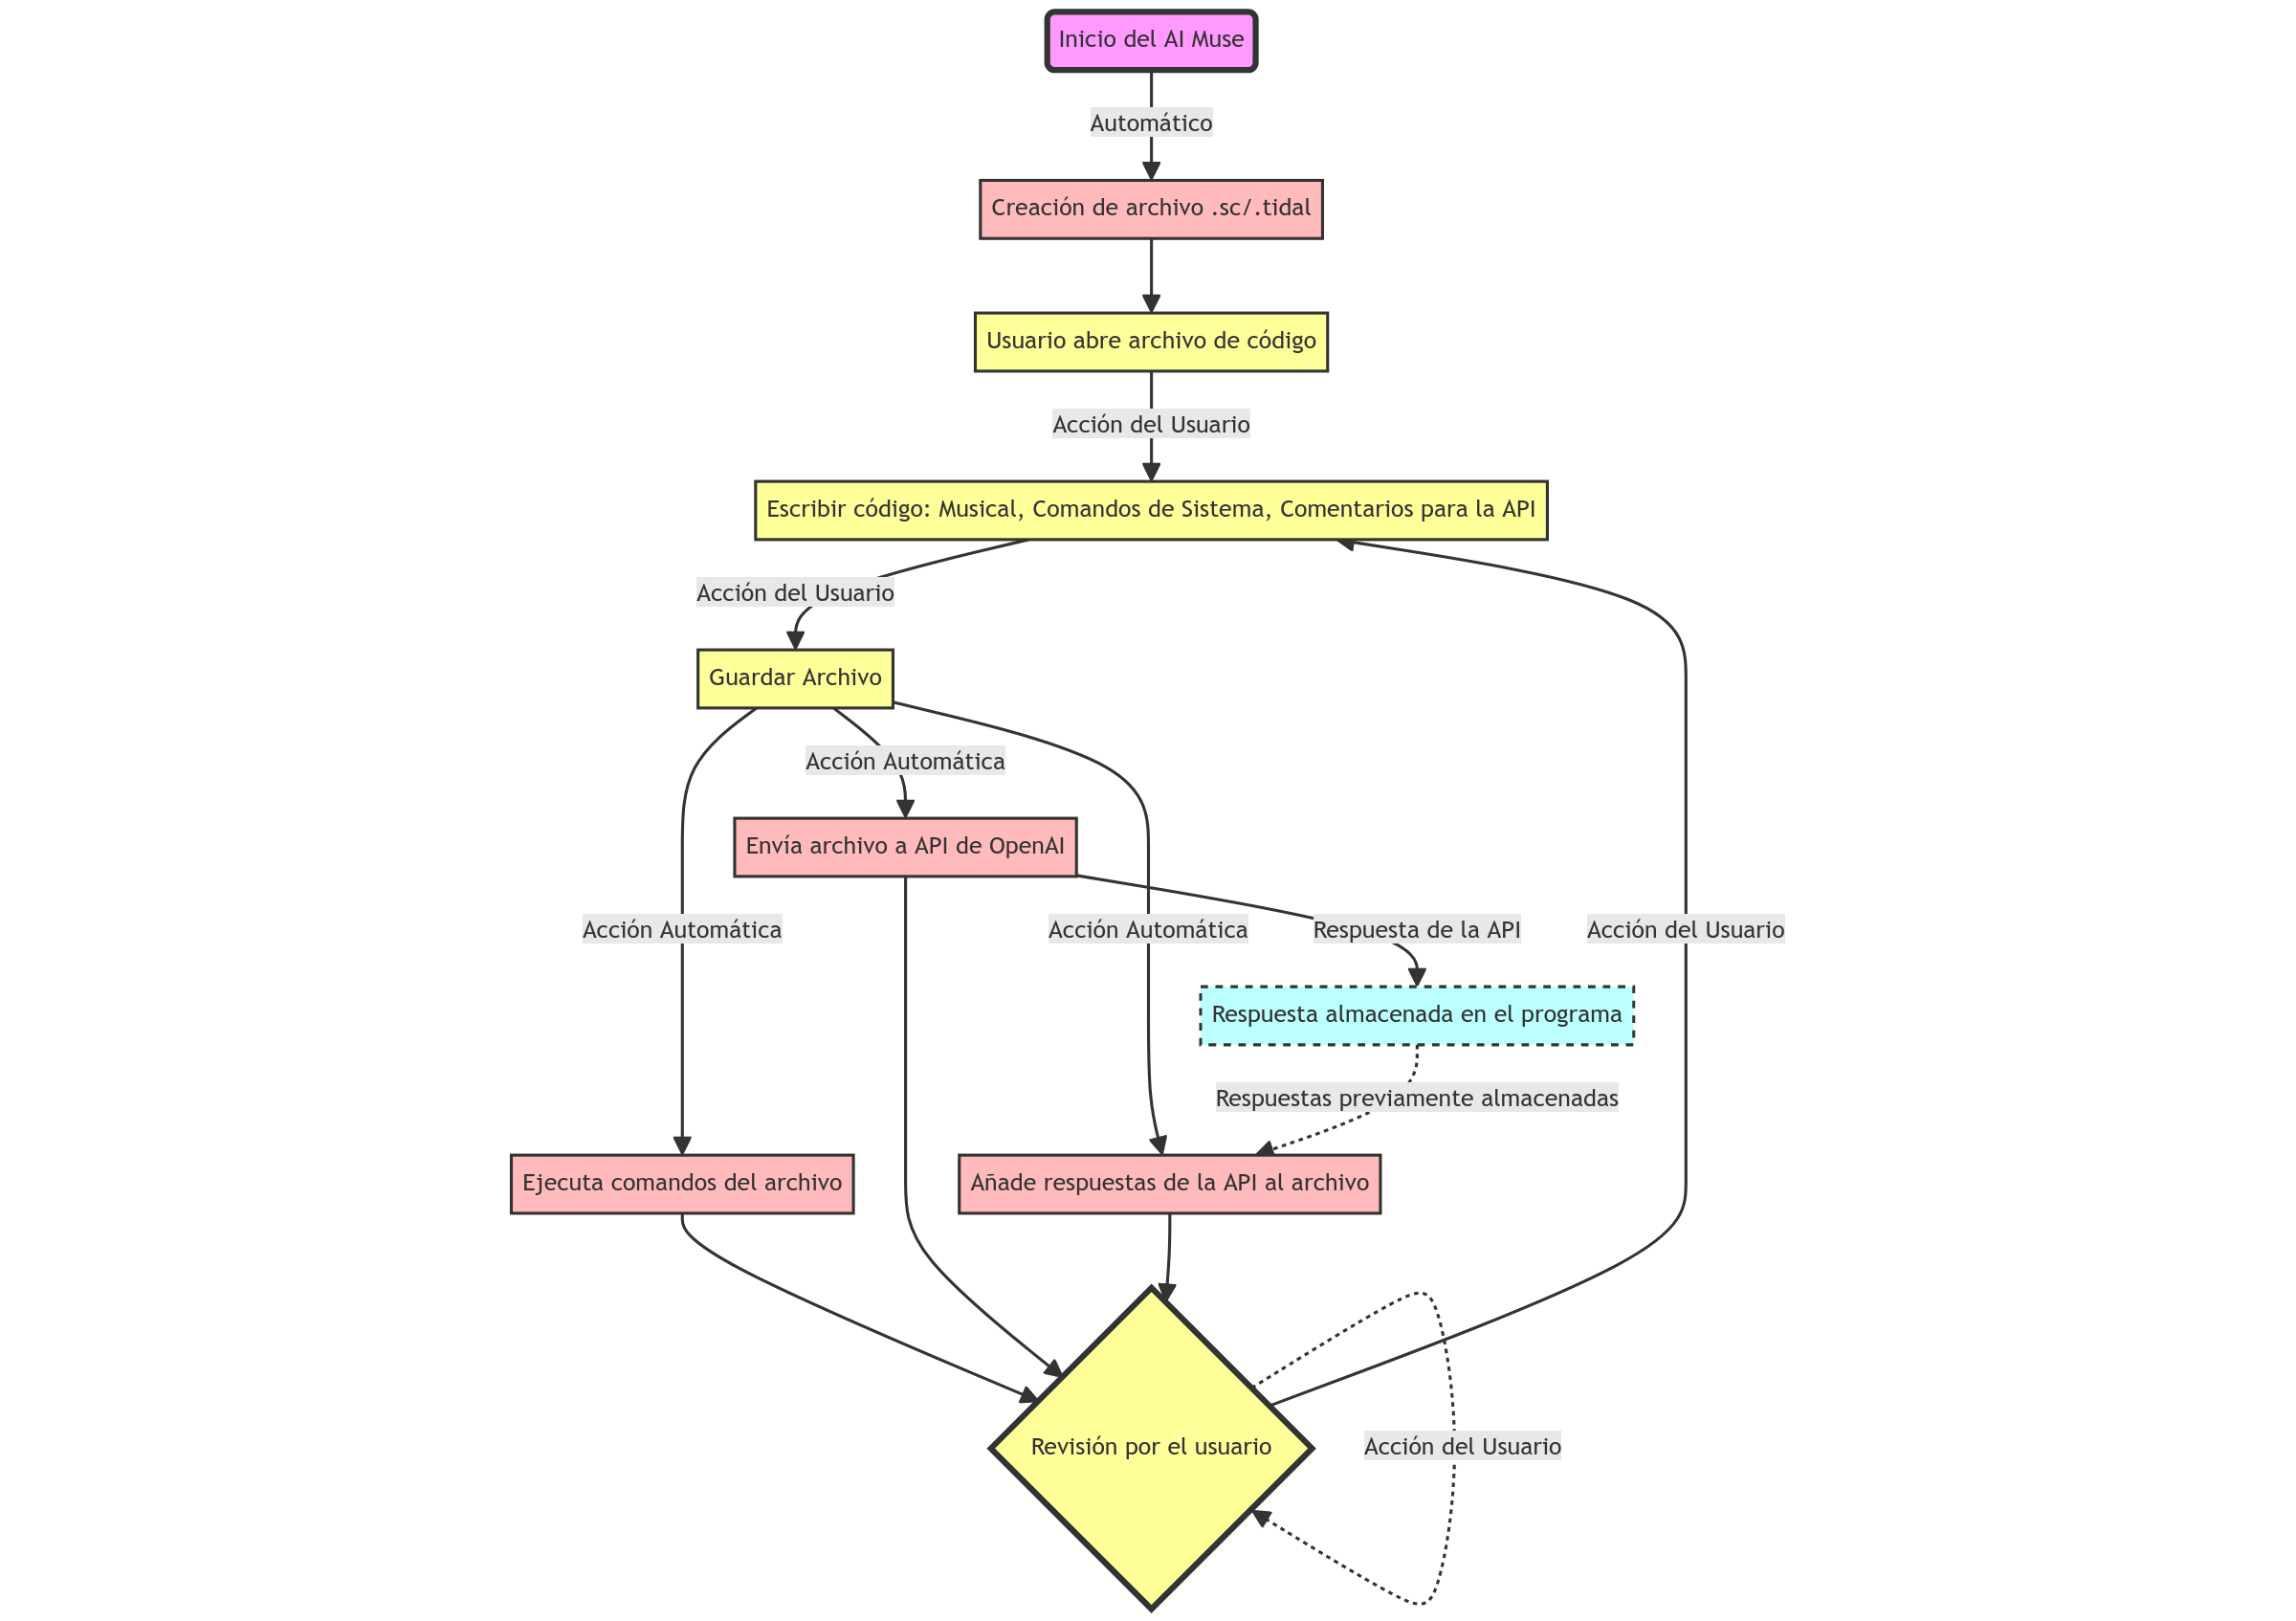
\includegraphics[width=1\textwidth]{./figuras/flujo_aimuse.png}
    \source{\propio}
    \label{fig:ai_muse_flow}
\end{figure}

% Código generador del diagrama:
% Se contruye en https://mermaid.live/
% https://mermaid.live/edit#pako:eNqNU8tu2zAQ_JWFclEAOQXqXqICBWRJtgXDaNGkJ7uHNbmK2VKiQFJuA9uf1EORT_CPlXr4lQJFdSDI3Zmd4VK79Zji5IXek8ZqDY_JsgT3RX5WCiYUcJIQZTCvDd3CYPBh18ZxByM_1oRMHF5KBwLUbC02Cu4Me3NnBUd521UaNSyI_S-mRu0K4kqf0Y7IDi9cPKkeHbfoxE8N02Il9DEdNg4EQxlArAosuTIN-UEYSwW2QSptI2CgQo0gEaJPWV81aaum_sRZ4Kgh6uT7bNpmx4v0G7HaIrCzgDw6_XoJnSzScnP4hadrtFqNn48VlVF2BZ4uosNvdDlNpqrJWGydd_4AXyuMW1K2_UwbYdrmVkqDM1J3_dt3sEkH6w7Ty0PWvtJccZG7fh37t4PkMn266jE78_srGVUKrhpfhvTGbXXb57oiHSspBScNCh6bB4b4mUkyfRdn3ct1h25lEo1JKAfR_Uu5kDK8ye_zwFitvlN4MxwO-_3gh-B2Hb6rfr5_RUbmuGVPXq3-QX77N5kTc2080fP8_n-0L4pA1Lu_rAyjIA6SIA3GwSSY9g6vANlJ-So8O2O9wCtIFyi4G75tA1p6dk0FLb3QbTnlWEu79Jbl3kGxturhuWReaHVNgVdXHC0lAt3YFl6YozQuSlxYpefdQLdzvf8DThJCbw

% graph TD
%     A(Inicio del AI Muse) -->|Automático| B[Creación de archivo .sc/.tidal]
%     B --> C[Usuario abre archivo de código]
%     C -->|Acción del Usuario| D[Escribir código: Musical, Comandos de Sistema, Comentarios para la API]
%     D -->|Acción del Usuario| E[Guardar Archivo]
%     E -->|Acción Automática| F[Ejecuta comandos del archivo]
%     E -->|Acción Automática| G[Envía archivo a API de OpenAI]
%     G -->|Respuesta de la API| K[Respuesta almacenada en el programa]
%     E -->|Acción Automática| H[Añade respuestas de la API al archivo]
%     K -.->|Respuestas previamente almacenadas| H
%     F --> I{Revisión por el usuario}
%     G --> I
%     H --> I
%     I -->|Acción del Usuario| D
%     I -.->|Acción del Usuario| I
    
%     classDef inicio fill:#f9f,stroke:#333,stroke-width:4px;
%     classDef accion fill:#bbf,stroke:#333,stroke-width:2px;
%     classDef decision fill:#ff9,stroke:#333,stroke-width:4px;
%     classDef almacenado fill:#bff,stroke:#333,stroke-width:2px,stroke-dasharray: 5, 5;
%     classDef usuario fill:#ff9,stroke:#333,stroke-width:2px;
%     classDef automatico fill:#fbb,stroke:#333,stroke-width:2px;
    
%     class A inicio;
%     class B automatico;
%     class C,D,E usuario;
%     class F,G,H automatico;
%     class I decision;
%     class K almacenado;
%     linkStyle 0,2,3,10,11 stroke:#333,stroke-width:2px;



\section{Archivo de configuración y comandos}

La Figura \ref{fig:json} muestra una configuración concreta para el archivo \texttt{config.json} \emph{AI Muse}. Este archivo, en formato JSON, será cargado al ejecutar el programa y contiene toda la información relevante en cuanto al lenguaje musical, modelo, hiperparámetros y otras opciones referentes a la propia aplicación, como el tiempo que ha de pasar entre dos peticiones. La Tabla \ref{table:json_comandos} muestra una breve descripción de estos parámetros, así como su traducción a comandos dentro de la propia aplicación.




\begin{table}[htbp]
    \centering
    \caption{Descripción de la configuración del archivo \texttt{config.json} y de sus correspondientes comandos.}
    \label{tab:config-description}
    % \setstretch{1}
    \fontsize{9.5pt}{11pt}\selectfont
    \begingroup
    \rowcolors{2}{azul_unir_soft}{white}
    \begin{tabularx}{\linewidth}{llXl}
        \toprule
        \rowcolor{azul_unir} % Aplica el color azul_unir al encabezado de la tabla
        \textbf{Clave} & \textbf{Valores posibles} & \textbf{Efecto}& \textbf{Ejemplo de uso en comando} \\
        \midrule
    % Tus filas aquí
    mode\_tidal\_supercollider & tidal/sclang & Modo de operación para TidalCycles o SuperCollider  & set mode tidal \\
    create\_log\_file & \textcolor{truecolor}{true}/\textcolor{falsecolor}{false} & Activa o desactiva la creación de archivos de registro  & - \\
    ghci\_path & \textcolor{pathcolor}{./ruta/a/ghci} & Ruta al ejecutable ghci  & - \\
    only\_system\_commands & \textcolor{truecolor}{true}/\textcolor{falsecolor}{false} & Restringe a comandos del sistema  & - \\
    supercollider\_on & \textcolor{truecolor}{true}/\textcolor{falsecolor}{false} & Enciende o apaga SuperCollider  & - \\
    sclang\_path & \textcolor{pathcolor}{./ruta/a/sclang} & Ruta al ejecutable sclang  & - \\
    boot\_tidal\_path & \textcolor{pathcolor}{/ruta/a/BootTidal.hs} & Ruta al archivo de arranque de Tidal  & - \\
    api\_enabled & \textcolor{truecolor}{true}/\textcolor{falsecolor}{false} & Activa o desactiva la API  & set api\_enabled \textcolor{truecolor}{true} \\
    bot\_mode & assistant/chat & Establece el modo del bot  & - \\
    assistant\_id & ID & ID del asistente  & - \\
    assistant\_retrieval\_folder & \textcolor{pathcolor}{./ruta/a/carpetas} & Ruta a la carpeta de recuperación  & - \\
    api\_key\_file & \textcolor{pathcolor}{apikey.txt} & Archivo con la clave de la API  & - \\
    system\_prompt\_file & \textcolor{pathcolor}{./ruta/a/system\_prompts} & Archivo de prompt del sistema  & - \\
    model & gpt-4-1106-preview/otro & Modelo de lenguaje utilizado  & - \\
    temperature & \textcolor{numbercolor}{0.0-2.0} & Temperatura para la generación de texto  & set temperature \textcolor{numbercolor}{0.7} \\
    max\_tokens & \textcolor{numbercolor}{Número entero} & Número máximo de tokens por generación  & set max\_tokens \textcolor{numbercolor}{256} \\
    top\_p & \textcolor{numbercolor}{0.0-1.0} & Ajusta la probabilidad de tomar caminos menos probables  & set top\_p \textcolor{numbercolor}{0.9} \\
    frequency\_penalty & \textcolor{numbercolor}{Número} & Penalización por frecuencia de tokens  & set frequency\_penalty \textcolor{numbercolor}{0.5} \\
    presence\_penalty & \textcolor{numbercolor}{Número} & Penalización por presencia de tokens  & set presence\_penalty \textcolor{numbercolor}{0.5} \\
    wait\_time\_before\_api & \textcolor{numbercolor}{Segundos} & Tiempo de espera antes de llamar a la API  & set wait\_time\_before\_api \textcolor{numbercolor}{10} \\
    wait\_time\_after\_api & \textcolor{numbercolor}{Segundos} & Tiempo de espera después de llamar a la API  & set wait\_time\_after\_api \textcolor{numbercolor}{10} \\
    \bottomrule
\end{tabularx}
\endgroup
\source{\propio}
\label{table:json_comandos}
\end{table}
    


\begin{figure}[H]
    \caption[Ejemplo de archivo de configuración \texttt{config.json} de AI Muse]{Ejemplo de archivo de configuración \texttt{\emph{config.json}} de AI Muse. Los valores de cada clave pueden ser modificados directamente en el archivo o por medio de comandos. En este caso, el programa creará música en Tidal Cycles y utiliza un Assistant (RAG) previamente creado con una ID determinada. El modelo es GPT-4. El número de tokens por petición-respuesta es de 256.}
    \centering
% \begin{mdframed}
\setstretch{1} % Esto establece el interlineado a sencillo
\begin{lstlisting}[language=json, numbers=none]
{
    "mode_tidal_supercollider": "tidal",
    "create_log_file": false,
    "ghci_path": "ghci",
    "only_system_commands": false,
    "supercollider_on": false,
    "sclang_path": "sclang",
    "boot_tidal_path": "/usr/share/haskell-tidal/BootTidal.hs",
    "api_enabled": false,
    "bot_mode": "assistant",
    "assistant_id": "asst_9Km6Fd3xywD4tGGY4yZzSEiw",
    "assistant_retrieval_folder": "./assistants/tidal_livecoding/retrieval_files/",
    "api_key_file": "apikey.txt",
    "system_prompt_file": "./assistants/tidal_livecoding/system_prompts/system_prompt_01",
    "model": "gpt-4-1106-preview",
    "temperature": 1,
    "max_tokens": 256,
    "top_p": 1,
    "frequency_penalty": 0,
    "presence_penalty": 0,
    "wait_time_before_api": 20,
    "wait_time_after_api": 20
}
\end{lstlisting}
% \end{mdframed}
    \source{\propio}
    \label{fig:json}
\end{figure}


% Explicar el sistema de archivos, especialmente el relativo a cómo debe configurarse la carpeta de un asistente, los prompts, etc.



\section{Resultados del uso de \emph{AI Muse}}

Como era de esperar, la automatización de los diálogos con el sistema del \gls{llm} permitió una interacción más fluida que en etapas previas, así como la concentración de la atención del usuario únicamente en cuestiones musicales. La música se produce ahora de forma sincrónica a la interacción usuario-\gls{llm}, lo cual se llega a percibir como una auténtica colaboración humano-máquina. Máxime cuando es posible comunicarse con comentarios en lenguaje natural durante el acto performativo.

Especial cuidado se puso en los prompts de sistema, ya que estos deben compendiar en el mínimo de tokens la finalidad de la conversación con el \gls{llm}, así como el formato esperado de sus respuestas para ser procesadas adecuadamente por el programa. En la Figura \ref{fig:system_prompts_aimuse} se muestran sendos prompts de sistema para Tidal Cycles y para SuperCollider, los cuales fueron utilizados con éxito en la práctica.

\begin{figure}[H]
    \caption[Prompts de sistema de AI Muse]{Prompts de sistema de AI Muse para (\textbf{a}) SuperCollider y (\textbf{b}) Tidal Cycles. Estos prompts están diseñados para que el \gls{llm} responda únicamente con código musical breve a partir del contexto del archivo completo y sus comentarios.}
    \centering
    \begin{subfigure}{.9\textwidth}
        \centering
    \begin{mdframed}
        \setstretch{1}
        \fontsize{9.5pt}{11pt}\selectfont
        Cada vez que se te escriba, debes devolver una sentencia de SuperCollider, o modificar una ya existente en el código.
        \setlength{\parskip}{6pt}

Responderás con una única sentencia que continúe el contexto proporcionado por la conversación, a modo de sesión de Live Coding.

No incluyas texto o comentarios.

Técnicamente, tus patrones no han de ser complejos, para asegurar que no contienen bugs.

Artísticamente, se busca en tus patrones: imaginación, patrones atípicos, texturas sin explorar, etc. No se espera de ti: repetición de códigos típicos. Lo que se oye ha de ser poco percusivo, no ha de recordar a una batería. Es música experimental y ambiental. Juega con sonidos no reconocibles, transformados como solo tú sabes hacer...

Busca que su resultado sonoro sea complejo.

Ten en cuenta que el resultado sonoro sea audible psicoacústicamente, especialmente si modificas mucho el sonido.

El usuario te pasa el archivo actual.

Tus bloques o sentencias del código llevan un comentario con el nombre del modelo que lo ha creado para que los reconozcas (tú no tienes que ponerlo, los indica el usuario).

Si modificas un patrón existente, cambialo sólo un poco, como haría un livecoder.

Utiliza sólo estructuras de live coding: Pbindef, Ndef, y objetos modificables en caliente. Crea tus SynthDefs.

Cuestiones técnicas: Si creas o modificas un SynthDef, no olvides añadir condición de terminación.

Devuelve un único bloque o sentencia.
    \end{mdframed}
        \caption{Prompt de sistema para SuperCollider}
      \end{subfigure}

    \vspace{5mm} % Añade espacio vertical entre las filas

      \begin{subfigure}{.9\textwidth}
        \centering
    \begin{mdframed}
        \setstretch{1}
        \fontsize{9.5pt}{11pt}\selectfont
        Cada vez que se escriba, debes devolver una sentencia de patrones de Tidal Cycles o modificación de uno existente.
        \setlength{\parskip}{6pt}

Responderás con una única sentencia que continúe el contexto proporcionado por la conversación, a modo de sesión de Live Coding.

No incluyas texto o comentarios.

Técnicamente, tus patrones no han de ser complejos, para asegurar que no contienen bugs.

Artísticamente, se busca en tus patrones: imaginación, patrones atípicos, texturas sin explorar, etc. No se espera de ti: repetición de códigos típicos. Lo que se oye ha de ser poco percusivo, no ha de recordar a una batería. Es música experimental y ambiental. Juega con sonidos estirados, llenos de eventos... transformados como solo tú sabes hacer...

Busca que su resultado sonoro sea complejo.

Ten en cuenta que el resultado sonoro sea audible psicoacústicamente, especialmente si modificas mucho el sonido.

El usuario te pasa el archivo actual.

Tú te ocuparás de algún patrón aún no creado (d1, d2, d3...), excepto si el usuario te pide que modifiques uno existente. Una vez existan 3 patrones tuyos, no crees más. Solo modifica los existentes.

Si modificas un patrón existente, cámbialo solo un poco, como haría un livecoder.

Cuestiones técnicas: no uses valores altos de room o sz, que pueden dar lugar a problemas de feedback.

Devuelve un único patrón. No uses ``` para formatear código.
    \end{mdframed}
        \caption{Prompt de sistema para Tidal Cycles}
      \end{subfigure}
    
    \source{\propio}
    \label{fig:system_prompts_aimuse}
\end{figure}

Se ha detectado una tenencia del \gls{llm} a imitar los patrones ya existentes en la conversación, si bien, por medio de comentarios es posible provocar más originalidad en sucesivas respuestas. Por esta razón, es interesante aplicar la técnica de prompting de \emph{few-shot} para dirigir el inicio de la improvisación colaborativa. 

No se ha hallado, sin embargo, una diferencia importante entre usar el modelo en modo \texttt{chat} o en modo \texttt{assistant}. Sin embargo, esto debería estudiarse con mayor detenimiento en función de unas cuidadas configuraciones de asistentes y de sus archivos de base de datos.

Este tipo de interacción se ha mostrado, en todo caso, muy prometedora de cara a la generación musical interactiva. Las aportaciones atómicas que se piden al \gls{llm} por medio de la API lo hacen muy adecuado como banco de pruebas tanto con los servicios de OpenAI, como eventualmente otros modelos, incluso open source.

